\chapter{Kiến trúc phần cứng}
\label{ch:arch}

\section{Tổng quan hệ thống}
Hình~\ref{fig:block} cho thấy kiến trúc tổng thể. CPU RISC-V (PicoRV32 \cite{picorv32} trong mô phỏng, Nios~V \cite{niosv} trên DE10-Nano) truy cập bộ tăng tốc như một vùng nhớ 64\,KiB qua giao diện tớ Avalon-MM \cite{avalonspec} 32 bit. Bên trong \code{npu\_avmm} có: bộ đệm trọng số (thực chất là các thanh ghi trọng số của mảng), bộ đệm kích hoạt ABUF, mảng systolic \code{sa\_top}, bộ đệm tích lũy CBUF (INT32), khối hậu xử lý, bộ đệm kết quả QBUF (INT8), các thanh ghi cấu hình và một bộ tuần tự (sequencer) đơn giản. Các tham số thiết kế: $N$ (kích thước mảng, bội của 4) và \code{DEPTH}$=64$ (số hàng tối đa của một lượt chạy).

\begin{figure}[H]
  \centering
  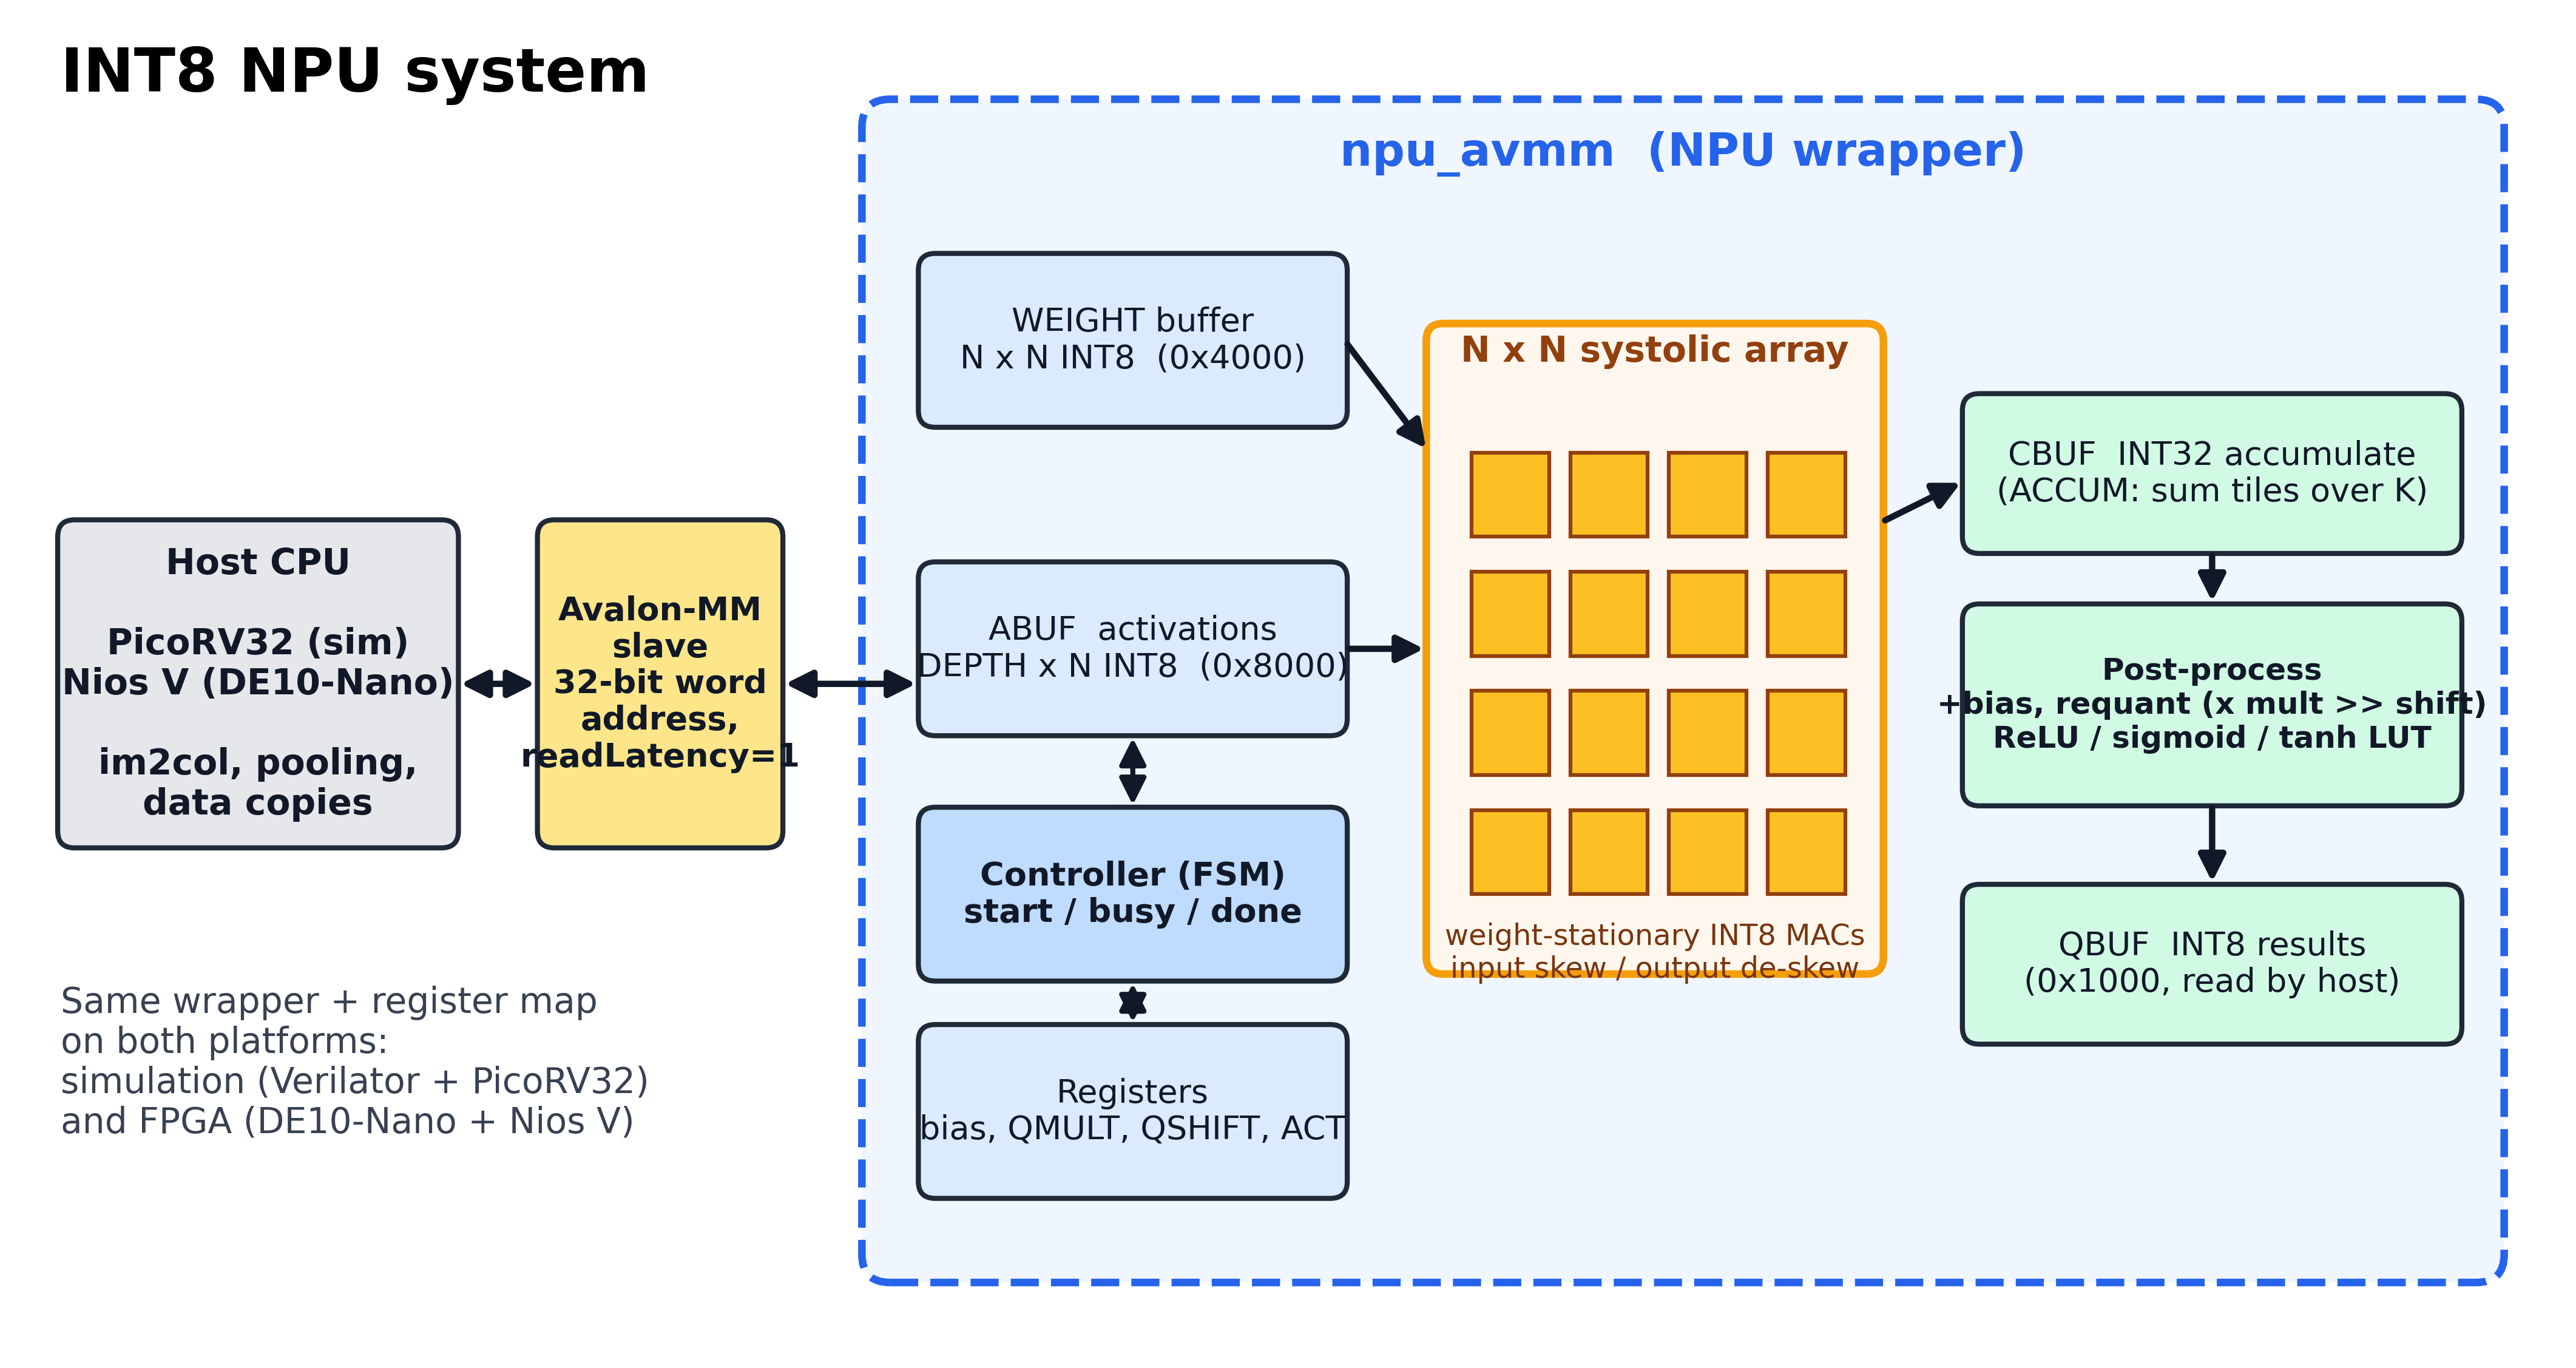
\includegraphics[width=0.95\linewidth]{d_block_diagram.png}
  \caption{Sơ đồ khối hệ thống: CPU host, cầu Avalon-MM, wrapper \code{npu\_avmm} với các bộ đệm, mảng systolic $N\times N$ và khối hậu xử lý (hình vẽ cho $N=4$).}
  \label{fig:block}
\end{figure}

Phân cấp RTL gồm bốn mô-đun (Bảng~\ref{tab:rtl-modules}).

\begin{table}[H]
  \centering
  \caption{Các mô-đun RTL}
  \label{tab:rtl-modules}
  \begin{tabularx}{\linewidth}{llX}
    \toprule
    Tệp & Dòng & Chức năng \\
    \midrule
    \code{rtl/pe.sv} & 21 & PE weight-stationary: thanh ghi kích hoạt 8 bit và tổng riêng 32 bit \\
    \code{rtl/delay.sv} & 25 & đường trễ $D$ chu kỳ có tham số ($D=0$ là dây nối) \\
    \code{rtl/sa\_top.sv} & 69 & mảng $N\times N$, thanh ghi trọng số, skew/de-skew, trễ \code{out\_valid} \\
    \code{rtl/npu\_avmm.sv} & 221 & wrapper Avalon-MM: thanh ghi, ABUF/CBUF/QBUF, sequencer, hậu xử lý \\
    \code{rtl/lut\_tables.svh} & (sinh) & hàm \code{lut\_sig}, \code{lut\_tanh} do \code{gen\_lut.py} sinh \\
    \bottomrule
  \end{tabularx}
\end{table}

\section{Phần tử xử lý (PE)}
PE (Đoạn mã~\ref{lst:pe}) là một khối tổ hợp nhân $8\times8$ có dấu, một bộ cộng 32 bit và hai thanh ghi. Trọng số $w$ không nằm trong PE mà là một thanh ghi của \code{sa\_top} được nối thẳng vào PE, nên PE không cần tín hiệu nạp trọng số. Ở mỗi sườn lên: $a_\text{out}\leftarrow a_\text{in}$ và $\text{psum}_\text{out}\leftarrow \text{psum}_\text{in}+a_\text{in}\cdot w$. Tích $a\cdot w$ nằm trong $[-16256, 16384]$ (cần 16 bit), được mở rộng dấu lên 32 bit.

\begin{lstlisting}[style=codesv, caption={PE weight-stationary (\code{rtl/pe.sv}, rút gọn)}, label={lst:pe}]
always_ff @(posedge clk or negedge rst_n) begin
    if (!rst_n) begin
        a_out    <= '0;
        psum_out <= '0;
    end else begin
        a_out    <= a_in;
        psum_out <= psum_in + 32'(a_in * w);
    end
end
\end{lstlisting}

\begin{figure}[H]
  \centering
  \begin{tikzpicture}[>={Stealth[length=2mm]}, font=\small,
      reg/.style={draw, thick, fill=gray!25, minimum width=1.0cm, minimum height=0.55cm, font=\scriptsize}]
    \node[draw, dashed, rounded corners, minimum width=7.0cm, minimum height=4.6cm] (box) at (3.0,-0.6) {};
    \node[anchor=north west, font=\footnotesize\bfseries] at (box.north west) {PE$(i,j)$};
    \node[draw, thick, circle, minimum size=0.8cm] (mul) at (1.6,0.0) {$\times$};
    \node[draw, thick, circle, minimum size=0.8cm] (add) at (3.6,-1.2) {$+$};
    \node[reg] (ra) at (5.4,1.0) {reg 8b};
    \node[reg] (rp) at (3.6,-2.3) {reg 32b};
    \draw[->] (-1.4,1.0) node[left] {$a_\text{in}$} -- (ra.west);
    \draw[->] (0.6,1.0) |- (mul.west);
    \fill (0.6,1.0) circle (1.5pt);
    \draw[->] (ra.east) -- ++(1.2,0) node[right] {$a_\text{out}$};
    \draw[->] (1.6,-1.9) node[below, align=center, font=\scriptsize] {$w=W_{ij}$\\(thanh ghi trong \code{sa\_top})} -- (mul.south);
    \draw[->] (mul.east) -| node[pos=0.25, above, font=\scriptsize] {16b$\to$32b} (add.north);
    \draw[->] (4.8,2.2) node[above] {$\text{psum}_\text{in}$} -- (4.8,-1.2) -- (add.east);
    \draw[->] (add.south) -- (rp.north);
    \draw[->] (rp.south) -- ++(0,-0.7) node[below] {$\text{psum}_\text{out}$};
  \end{tikzpicture}
  \caption{Cấu trúc PE: một bộ nhân INT8, một bộ cộng INT32 và hai thanh ghi (màu xám). Kích hoạt đi ngang, tổng riêng đi dọc.}
  \label{fig:pe}
\end{figure}

\section{Mảng systolic \code{sa\_top}}
\subsection{Giao diện}
\begin{itemize}
  \item \textbf{Cổng ghi trọng số}: \code{w\_we}, \code{w\_widx}, \code{w\_wdata[31:0]}. Từ thứ $\text{idx}=i\cdot(N/4)+q$ chứa $W_{i,4q},\dots,W_{i,4q+3}$ (byte $b$ $\to$ cột $4q+b$). Như vậy một lần ghi bus nạp 4 trọng số, và cả khối $N\times N$ cần $N^2/4$ lần ghi (16 lần với $N=8$).
  \item \textbf{Luồng kích hoạt}: \code{in\_valid}, \code{a\_in[8N-1:0]} -- một hàng $A_{m,:}$ mỗi chu kỳ, phần tử $k$ ở bit $[8k+7:8k]$. Có thể có ``khoảng trống'' (chu kỳ \code{in\_valid}$=0$) giữa các hàng.
  \item \textbf{Luồng kết quả}: \code{out\_valid}, \code{c\_out[32N-1:0]} -- một hàng $C_{m,:}$ INT32.
\end{itemize}

\subsection{Skew, de-skew và độ trễ $2N-1$}
\label{sec:latency}
Hàng $i$ của đầu vào đi qua mô-đun \code{delay} với $D=i$; cột $j$ của đầu ra đi qua \code{delay} với $D=N-1-j$; tín hiệu \code{in\_valid} đi qua \code{delay} với $D=2N-1$ để thành \code{out\_valid}. Đặt chu kỳ $0$ là chu kỳ hàng $A_{m,:}$ có mặt ở \code{a\_in}. Theo Mục~\ref{sec:ws-example}, PE$(i,j)$ xử lý $A_{m,i}$ tại chu kỳ $m+i+j$ và thanh ghi kết quả của nó có giá trị từ chu kỳ $m+i+j+1$. Với hàng cuối $i=N-1$, tổng đầy đủ $C_{m,j}$ có ở đáy cột $j$ từ chu kỳ $m+N+j$. Sau de-skew $N-1-j$ chu kỳ:
\begin{equation}
  t_\text{out}(m) = m + N + j + (N-1-j) = m + 2N - 1,
\end{equation}
độc lập với $j$. Vậy \textbf{độ trễ từ \code{in\_valid} tới \code{out\_valid} là $2N-1$ chu kỳ} (7 với $N=4$, 15 với $N=8$) và thông lượng là một hàng mỗi chu kỳ. Điều này được xác nhận trên dạng sóng Verilator (Hình~\ref{fig:waveform}). Chi phí phần cứng của skew/de-skew là $\sum_{i}i=N(N-1)/2$ thanh ghi 8 bit và $N(N-1)/2$ thanh ghi 32 bit.

\begin{figure}[H]
  \centering
  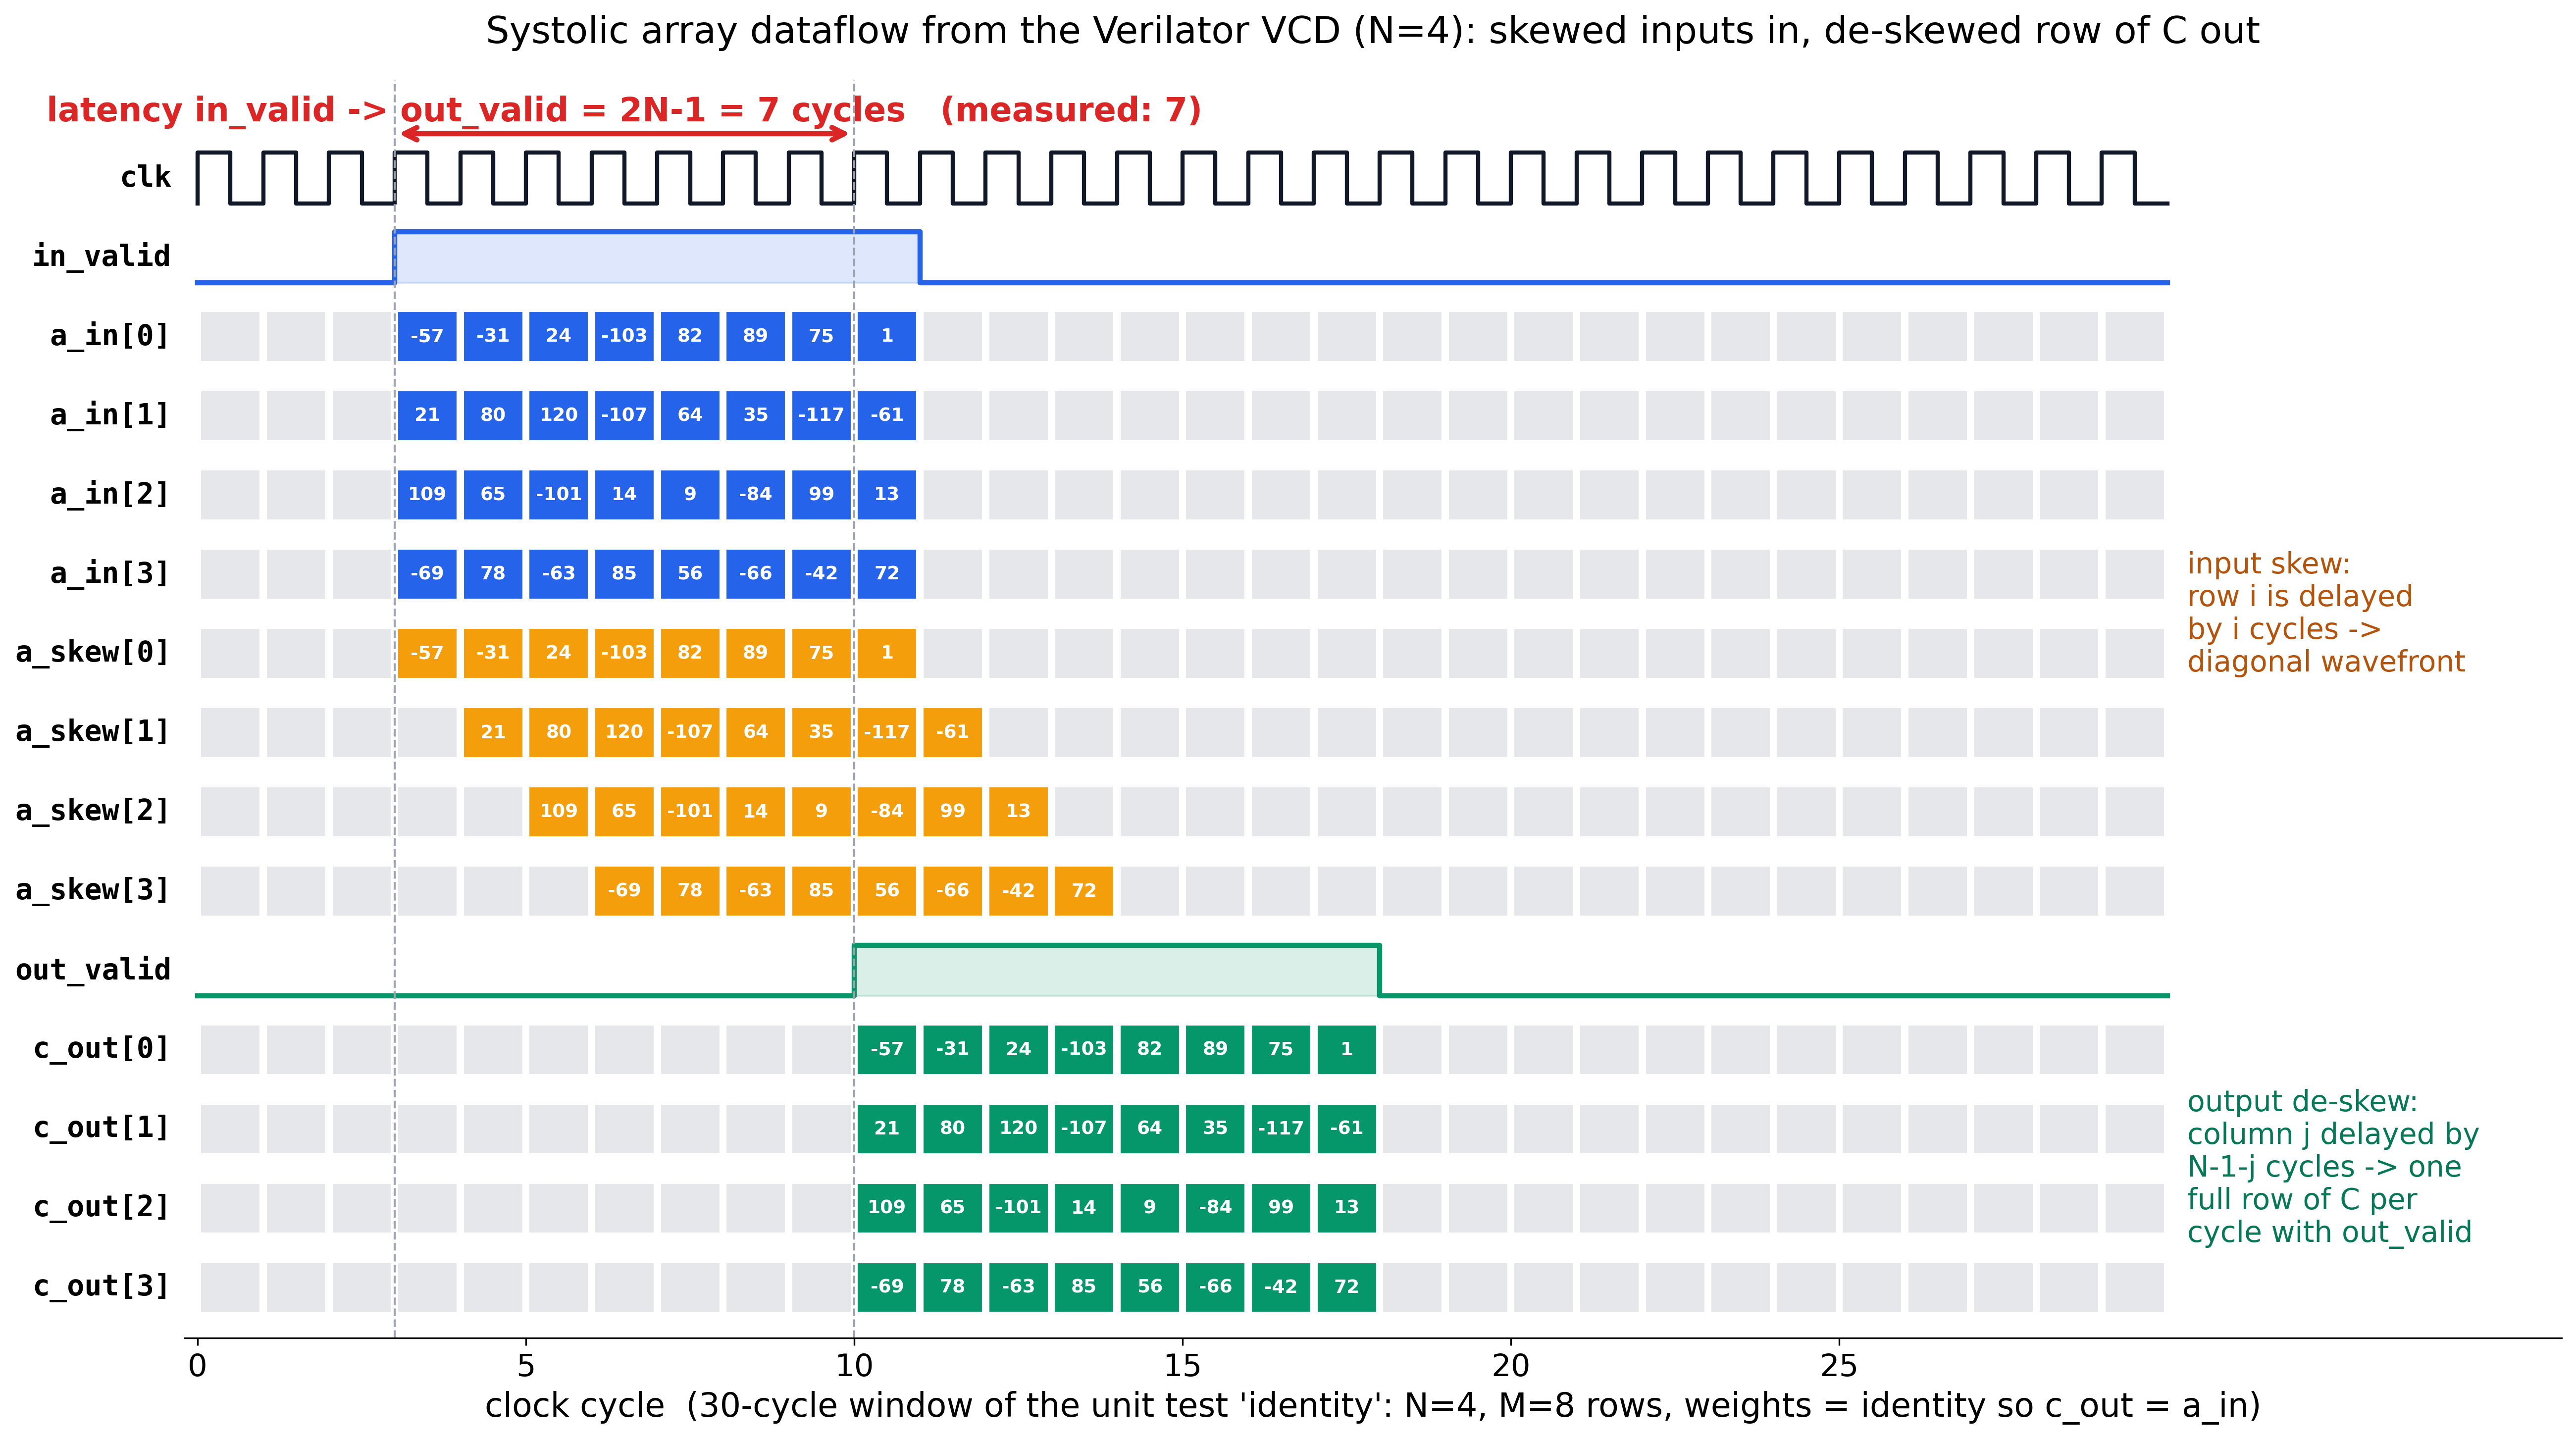
\includegraphics[width=\linewidth]{c_waveform_dataflow.png}
  \caption{Dạng sóng Verilator của unit test $N=4$ (\code{make wave N=4}): đầu vào \code{a\_in}, các hàng sau skew (mỗi hàng trễ thêm một chu kỳ), \code{in\_valid}, \code{out\_valid} trễ $2N-1=7$ chu kỳ và \code{c\_out} đã de-skew.}
  \label{fig:waveform}
\end{figure}

\subsection{Tài nguyên logic theo $N$}
Bảng~\ref{tab:sa-cost} đếm (theo RTL) các phần tử chính. Số bộ nhân tăng theo $N^2$; số thanh ghi trễ tăng theo $N^2/2$.

\begin{table}[H]
  \centering
  \caption{Phần tử chính của \code{sa\_top} theo $N$ (đếm từ RTL)}
  \label{tab:sa-cost}
  \begin{tabular}{lccc}
    \toprule
    Thành phần & Công thức & $N=4$ & $N=8$\\
    \midrule
    Bộ nhân $8\times8$ & $N^2$ & 16 & 64 \\
    Bộ cộng 32 bit & $N^2$ & 16 & 64 \\
    Thanh ghi trọng số (bit) & $8N^2$ & 128 & 512 \\
    Thanh ghi kích hoạt trong PE (bit) & $8N^2$ & 128 & 512 \\
    Thanh ghi tổng riêng trong PE (bit) & $32N^2$ & 512 & \num{2048} \\
    Thanh ghi skew (bit) & $8\cdot N(N-1)/2$ & 48 & 224 \\
    Thanh ghi de-skew (bit) & $32\cdot N(N-1)/2$ & 192 & 896 \\
    \bottomrule
  \end{tabular}
\end{table}

\section{Wrapper Avalon-MM \code{npu\_avmm}}
\subsection{Giao diện bus}
Wrapper là một tớ Avalon-MM với địa chỉ từ 14 bit (không gian 64\,KiB), dữ liệu 32 bit, \code{readLatency}$=1$ cố định, \code{waitrequest} luôn bằng 0. Mọi lệnh ghi được chấp nhận trong một chu kỳ; dữ liệu đọc xuất hiện ở chu kỳ ngay sau chu kỳ \code{read} cùng với \code{readdatavalid} (Hình~\ref{fig:avalon}). Thiết kế không có \code{byteenable}: mọi truy cập đều là từ 32 bit, nên driver luôn ghi đủ 4 byte.

\begin{figure}[H]
  \centering
  \begin{tikzpicture}[x=1.1cm, y=0.6cm, font=\footnotesize]
    \def\sig#1#2{\node[left] at (0,#1) {#2};}
    \sig{0}{clk}
    \foreach \k in {0,...,7} { \draw (\k,-0.3) -- (\k,0.3) -- (\k+0.5,0.3) -- (\k+0.5,-0.3) -- (\k+1,-0.3); }
    \sig{-1.5}{address}
    \draw (0,-1.2) -- (0.1,-1.2); \draw (0.1,-1.8) -- (0.1,-1.2) -- (1.9,-1.2) -- (1.9,-1.8) -- (0.1,-1.8);
    \node at (1,-1.5) {W:0x8000};
    \draw (2.1,-1.8) -- (2.1,-1.2) -- (3.9,-1.2) -- (3.9,-1.8) -- (2.1,-1.8);
    \node at (3,-1.5) {R:0x0004};
    \sig{-3}{write}
    \draw (0,-3.3) -- (0.1,-3.3) -- (0.1,-2.7) -- (1.1,-2.7) -- (1.1,-3.3) -- (8,-3.3);
    \sig{-4.5}{read}
    \draw (0,-4.8) -- (2.1,-4.8) -- (2.1,-4.2) -- (3.1,-4.2) -- (3.1,-4.8) -- (8,-4.8);
    \sig{-6}{readdatavalid}
    \draw (0,-6.3) -- (3.1,-6.3) -- (3.1,-5.7) -- (4.1,-5.7) -- (4.1,-6.3) -- (8,-6.3);
    \sig{-7.5}{readdata}
    \draw (3.1,-7.8) -- (3.1,-7.2) -- (4.1,-7.2) -- (4.1,-7.8) -- (3.1,-7.8);
    \node at (3.6,-7.5) {STATUS};
    \draw[dashed, gray] (1,0.5) -- (1,-8); \draw[dashed, gray] (3,0.5) -- (3,-8);
    \node[gray, above] at (1,0.5) {ghi chấp nhận};
    \node[gray, above] at (3.6,0.5) {dữ liệu đọc (latency 1)};
  \end{tikzpicture}
  \caption{Định thời Avalon-MM của \code{npu\_avmm}: ghi hoàn tất trong một chu kỳ; đọc có \code{readLatency}$=1$ và không có \code{waitrequest}.}
  \label{fig:avalon}
\end{figure}

\subsection{Bản đồ thanh ghi và bộ đệm}
Bảng~\ref{tab:regmap} là bản đồ địa chỉ (offset byte), lấy từ chú thích đầu tệp \code{rtl/npu\_avmm.sv}. Hai bit cao của địa chỉ từ chọn vùng: \code{00} thanh ghi/QBUF, \code{01} trọng số, \code{10} ABUF, \code{11} CBUF.

\begin{table}[H]
  \centering
  \caption{Bản đồ thanh ghi và bộ đệm của \code{npu\_avmm} (offset byte so với địa chỉ cơ sở)}
  \label{tab:regmap}
  \small
  \begin{tabularx}{\linewidth}{lllX}
    \toprule
    Offset & Tên & R/W & Mô tả \\
    \midrule
    \code{0x0000} & CTRL & W & bit0 START, bit1 CLEAR (xóa done/err), bit2 ACCUM (cộng vào CBUF thay vì ghi đè), bit3 QUANT (sau tích lũy chạy bias+requant+kích hoạt vào QBUF) \\
    \code{0x0004} & STATUS & R & bit0 busy, bit1 done, bit2 err ($M=0$ hoặc $M>\text{DEPTH}$) \\
    \code{0x0008} & M & RW & số hàng của lượt chạy, $1\dots\text{DEPTH}$ \\
    \code{0x000C} & CYCLES & R & số chu kỳ busy của lượt chạy cuối \\
    \code{0x0010} & INFO & R & \{DEPTH[15:0], N[15:0]\} \\
    \code{0x0014} & QMULT & W & hệ số $\mu$, 16 bit có dấu \\
    \code{0x0018} & QSHIFT & W & số bit dịch $\sigma$, $0\dots31$ \\
    \code{0x001C} & ACT & W & 0 không, 1 ReLU, 2 sigmoid LUT, 3 tanh LUT \\
    \code{0x0040}+$4j$ & BIAS[$j$] & W & bias INT32 của cột $j$ \\
    \code{0x1000} & QBUF & R & kết quả INT8; hàng $m$ byte $j$ tại $\code{0x1000}+4m(N/4)+j$ \\
    \code{0x4000} & WEIGHT & W & từ $i(N/4)+q$ = $W_{i,4q..4q+3}$ \\
    \code{0x8000} & ABUF & W & kích hoạt; hàng $m$ byte $k$ tại $\code{0x8000}+4m(N/4)+k$ \\
    \code{0xC000} & CBUF & R & tích lũy INT32, $C_{m,j}$ tại $\code{0xC000}+4(mN+j)$ \\
    \bottomrule
  \end{tabularx}
\end{table}

Ghi vào WEIGHT và ABUF bị bỏ qua khi \code{busy}$=1$ để tránh làm hỏng lượt chạy hiện tại. Dung lượng bộ đệm với \code{DEPTH}$=64$: ABUF và QBUF mỗi bộ $64\times8N$ bit (512\,B với $N=8$), CBUF $64\times32N$ bit (2\,KiB với $N=8$).

\subsection{Bộ tuần tự}
Một lượt chạy được kích hoạt bằng cách ghi \code{M} rồi ghi CTRL với bit START cùng các cờ ACCUM/QUANT. Nếu $M$ hợp lệ, \code{busy} lên 1 và mỗi chu kỳ sequencer đọc một hàng ABUF đưa vào mảng (\code{sent}), đồng thời mỗi khi \code{out\_valid} lên thì ghi một hàng vào CBUF (\code{recv}):
\begin{equation}
  \text{CBUF}[m] \leftarrow \begin{cases} \text{CBUF}[m] + C_{m,:} & \text{nếu ACCUM}\\ C_{m,:} & \text{ngược lại.}\end{cases}
\end{equation}
Nhờ cờ ACCUM, một GEMM có $K>N$ được chia thành $\lceil K/N\rceil$ lượt chạy liên tiếp với cùng các hàng $m$ nhưng khác khối trọng số; tổng $\sum_k$ được cộng dồn trong CBUF mà không cần CPU đọc kết quả trung gian. Chỉ lượt cuối có cờ QUANT.

Số chu kỳ busy của một lượt (đo bằng thanh ghi CYCLES và kiểm chứng ở Chương~\ref{ch:results}) là
\begin{equation}
  T_\text{busy}(M) = M + 2N + [\text{QUANT}],
  \label{eq:tbusy}
\end{equation}
gồm 1 chu kỳ đọc ABUF, $M-1$ chu kỳ đưa các hàng còn lại, $2N-1$ chu kỳ trễ của mảng, 1 chu kỳ ghi CBUF/kết thúc, và thêm 1 chu kỳ cho tầng đường ống hậu xử lý khi có QUANT. Ví dụ \code{gemm\_demo} $N=8$, $M=64$ đo được 80 chu kỳ $=64+16$.

\subsection{Khối hậu xử lý}
Khi cờ QUANT bật, khối hậu xử lý gồm hai tầng đường ống cho mỗi hàng kết quả:
\begin{enumerate}
  \item \textbf{Tầng 1} (cùng chu kỳ ghi CBUF): $p_j \leftarrow (\text{sum}_j + \text{bias}_j)\cdot\mu$, $N$ bộ nhân $32\times16$ có kết quả 48 bit, lưu vào thanh ghi \code{prod[j]}.
  \item \textbf{Tầng 2}: cộng hằng làm tròn $2^{\sigma-1}$, dịch phải số học $\sigma$ bit, bão hòa về $[-128,127]$, rồi chọn kích hoạt (không / ReLU / \code{lut\_sig} / \code{lut\_tanh}) và ghi một hàng vào QBUF.
\end{enumerate}
Công thức đúng như \eqref{eq:requant}. Hàm kích hoạt có thể khác nhau giữa các lượt chạy (thanh ghi ACT), nhờ đó các cột của LSTM thuộc cổng $g$ dùng tanh, các cột thuộc cổng $i,f,o$ dùng sigmoid (Chương~\ref{ch:sw}). LUT được tổng hợp thành logic tổ hợp (hàm \code{case} 256 nhánh); trên FPGA có thể chuyển thành ROM.

\section{Tích hợp trong SoC mô phỏng}
SoC mô phỏng (\code{soc/soc\_top.sv}) gồm PicoRV32 (RV32IM, bộ nhân nhanh, bộ chia, barrel shifter, bộ đếm chu kỳ 64 bit), 256\,KiB RAM, một cổng ``putchar'' và một cổng ``exit'' cho testbench, và một cầu chuyển giao diện bộ nhớ native của PicoRV32 sang Avalon-MM (Bảng~\ref{tab:socmap}). Lệnh đọc tới \NPU{} mất hai pha (phát \code{read}, chờ \code{readdatavalid}), lệnh ghi mất một chu kỳ bus.

\begin{table}[H]
  \centering
  \caption{Bản đồ bộ nhớ của SoC mô phỏng}
  \label{tab:socmap}
  \begin{tabular}{lll}
    \toprule
    Địa chỉ & Thiết bị & Ghi chú \\
    \midrule
    \code{0x0000\_0000} & RAM 256\,KiB & mã + dữ liệu, nạp từ \code{fw.hex} \\
    \code{0x1000\_0000} & putchar (W) & in ký tự ra log mô phỏng \\
    \code{0x1000\_0004} & exit (W) & kết thúc mô phỏng với mã thoát \\
    \code{0x2000\_0000} & \NPU{} (64\,KiB) & \code{npu\_avmm} qua cầu Avalon-MM \\
    \bottomrule
  \end{tabular}
\end{table}

Trên DE10-Nano, cùng mô-đun \code{npu\_avmm} được đóng gói thành một thành phần Platform Designer và nối vào Nios~V qua interconnect Avalon (Chương~\ref{ch:fpga}); driver chỉ cần đổi macro \code{NPU\_BASE}.
